\documentclass[12pt]{article}%
\usepackage{amsfonts}
\usepackage{fancyhdr}
\usepackage{comment}
\usepackage[a4paper, top=2.5cm, bottom=2.5cm, left=2.2cm, right=2.2cm]%
{geometry}
% \usepackage{times}
\usepackage{amsmath}
\usepackage{changepage}
\usepackage{amssymb}
\usepackage{graphicx}
\usepackage{url}
\setcounter{MaxMatrixCols}{30}
\newtheorem{theorem}{Theorem}
\newtheorem{acknowledgement}[theorem]{Acknowledgement}
\newtheorem{algorithm}[theorem]{Algorithm}
\newtheorem{axiom}{Axiom}
\newtheorem{case}[theorem]{Case}
\newtheorem{claim}[theorem]{Claim}
\newtheorem{conclusion}[theorem]{Conclusion}
\newtheorem{condition}[theorem]{Condition}
\newtheorem{conjecture}[theorem]{Conjecture}
\newtheorem{corollary}[theorem]{Corollary}
\newtheorem{criterion}[theorem]{Criterion}
\newtheorem{definition}[theorem]{Definition}
\newtheorem{example}[theorem]{Example}
\newtheorem{exercise}[theorem]{Exercise}
\newtheorem{lemma}[theorem]{Lemma}
\newtheorem{notation}[theorem]{Notation}
\newtheorem{problem}[theorem]{Problem}
\newtheorem{proposition}[theorem]{Proposition}
\newtheorem{remark}[theorem]{Remark}
\newtheorem{solution}[theorem]{Solution}
\newtheorem{summary}[theorem]{Summary}
\newenvironment{proof}[1][Proof]{\textbf{#1.} }{\ \rule{0.5em}{0.5em}}

\newcommand{\Q}{\mathbb{Q}}
\newcommand{\R}{\mathbb{R}}
\newcommand{\C}{\mathbb{C}}
\newcommand{\Z}{\mathbb{Z}}
\newcommand{\PARTIAL}[2]{\frac{\partial #1}{\partial #2}}
\renewcommand{\b}[1]{\boldsymbol{#1}}
\begin{document}

\title{CS280 Fall 2022 Assignment 1 \\ Part A}
\author{Basics \& MLP}
\maketitle

\paragraph{Name: Bingnan Li}

\paragraph{Student ID: 2020533092}

\newpage


%\subsubsection*{3. Gaussian Distributions (10 points)}
%Let $X\sim N(0,1)$ and $Y=WX$, where $p(W=-1)=p(W=1)=0.5$. It is clear that $X$ and $Y$ are not independent since $Y$ is a function of $X$. 
%\begin{itemize}
%	\item Show $Y\sim N(0,1)$
%	\item Show $cov[X,Y]=0$. hint: $cov[X,Y]=E[XY]-E[X]E[Y]$ and $E[XY]=E[E[XY|W]]$
%\end{itemize}
%Therefore, $X$ and $Y$ are uncorrelated and Gaussian, but they are dependent. Why?
\subsubsection*{1. \textit{Gradient descent for fitting GMM} (10 points).}
Consider the Gaussian mixture model
\[p(\mathbf{x}|\theta)=\sum_{k=1}^K \pi_k \mathcal{N}(\mathbf{x}|\boldsymbol{\mu}_k,\boldsymbol{\Sigma}_k)\]
\indent where $\pi_j\geq 0, \sum_{j=1}^K\pi_j = 1$. (Assume $\mathbf{x},\boldsymbol{\mu}_k\in \mathbb{R}^d,\boldsymbol{\Sigma}_k\in \mathbb{R}^{d\times d}$)
\vspace{1em}
\\
 Define the log likelihood as
\[ l(\theta) = \sum_{n=1}^N \log p(\mathbf{x}_n|\theta)
\]
 Denote the posterior responsibility that cluster $k$ has for datapoint $n$ as follows:
\[
r_{nk}:=p(z_n=k|\mathbf{x}_n,\theta) = \frac{\pi_k\mathcal{N}(\mathbf{x}_n|\boldsymbol{\mu}_k,\boldsymbol{\Sigma}_k)}{\sum_{k'}\pi_{k'}\mathcal{N}(\mathbf{x}_n|\boldsymbol{\mu}_{k'},\boldsymbol{\Sigma}_{k'})}
\]
\\
(a) Show that the gradient of the log-likelihood wrt $\boldsymbol{\mu}_k$ is
	\[ \frac{d}{d\boldsymbol{\mu}_k}l(\theta) = \sum_n r_{nk}\boldsymbol{\Sigma}_k^{-1}(\mathbf{x}_n-\boldsymbol{\mu}_k)
	\]
	\vspace{1em}
    \begin{proof}
        By the {\it chain rule}, we have 
        \begin{align*}
            \PARTIAL{l(\theta)}{\b{\mu}_k}
            &=\sum_{n=1}^N \frac{1}{p(\b{x}_n|\theta)}\PARTIAL{p(\b{x}_n|\theta)}{\b{\mu}_k}\\
            &=\sum_{n=1}^N \frac{1}{p(\b{x}_n|\theta)}\PARTIAL{\pi_k\mathcal{N}(\b{x}_n|\b{\mu}_k,\b{\Sigma}_k)}{\b{\mu}_k}\\
            &=\sum_{n=1}^N \frac{\pi_k\mathcal{N}(\b{x}_n|\b{\mu}_k,\b{\Sigma}_k)}{p(\b{x}_n|\theta)}\PARTIAL{(-\frac{1}{2}(\b{x}_n-\b{\mu}_k)^T\b{\Sigma}^{-1}(\b{x}_n-\b{\mu}_k))}{\b{\mu}_k}\\
            &=\sum_{n=1}^N r_{nk}\b{\Sigma}^{-1}(\b{x}_n-\b{\mu}_k)
        \end{align*}
    \end{proof}
	\vspace{1em}

	(b) Derive the gradient of the log-likelihood wrt $\pi_k$ without considering any constraint on $\pi_k$. (bonus 2 points: with constraint $\sum_k\pi_k=1$.)
	\vspace{1em}

    \begin{proof}
        For the case without any constriant on $\pi_k$, by the {\it chain rule}, we have:
        \begin{align*}
            \PARTIAL{l(\theta)}{\pi_k}
            &=\sum_{n=1}^N \frac{1}{p(\b{x}_n|\theta)}\PARTIAL{p(\b{x}_n|\theta)}{\pi_k}\\
            &=\sum_{n=1}^N \frac{1}{p(\b{x}_n|\theta)}\mathcal{N}(\b{x}_n|\b{\mu}_k,\b{\Sigma}_k)\\
            &=\sum_{n=1}^N \frac{r_{nk}}{\pi_k}
        \end{align*}
    \end{proof}
	\vspace{1em}

\pagebreak

\subsubsection*{2. \textit{Sotfmax \& Computation Graph} (10 points).}
Recall that the softmax function takes in a vector $(z_1, \dots , z_D)$ and returns a
vector $(y_1, \dots , y_D)$. We can express it in the following form:
\begin{equation*}
    \begin{split}
    r = \sum_j e^{z_j}   \qquad y = \frac{e^{z_j}}{r}
\end{split}
\end{equation*}
(a) Consider $D = 2$, i.e. just two inputs and outputs to the softmax. Draw the
computation graph relating $z_1$, $z_2$, $r$, $y_1$, and $y_2$.
\vspace{1em}\\
{\bf Solution:}
\begin{figure}[h]
    \begin{center}
        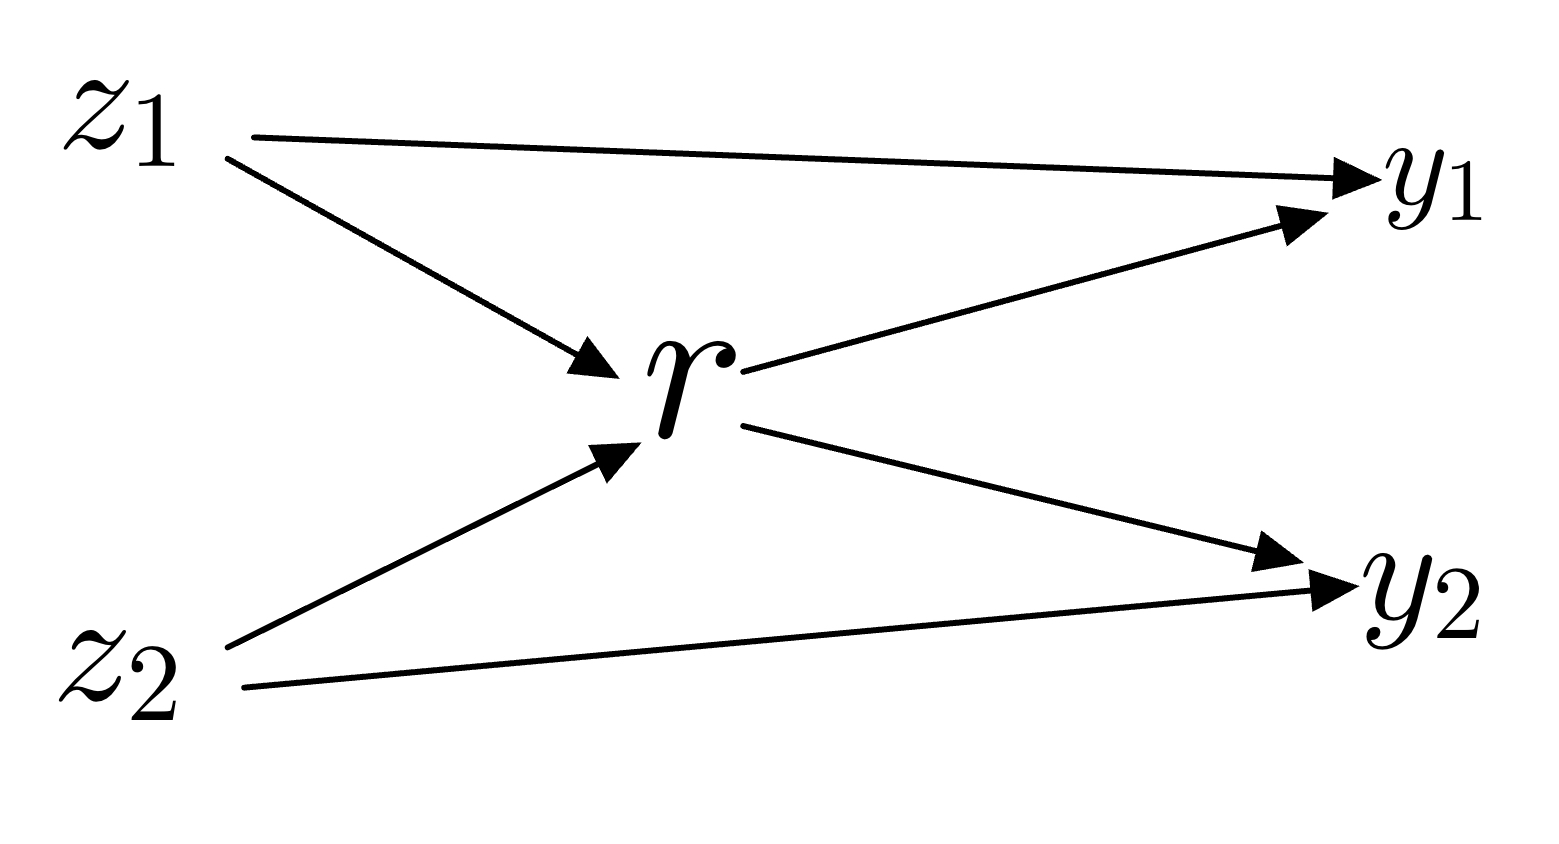
\includegraphics[width=0.5\columnwidth]{img/Q2(a).jpeg}        
    \end{center}
\end{figure}


(b) Determine the backprop updates for computing the $\bar{z_j}$ when given the $\bar{y_i}$.
You need to justify your answer. (You may give your answer either for
$D = 2$ or for the more general case.)\\
{\bf Solution:}
\par By the {\it chain rule} and the forward precess, we have the backprop updates as follows:
\begin{align*}
    \bar{r} &= \sum_{i=1}^D \bar{y}_i \PARTIAL{y_i}{r} = -\sum_{i=1}^D\bar{y}_i\frac{e^{z_i}}{r^2}\\
    \bar{z}_i &= \bar{y}_i\PARTIAL{y_i}{z_i} + \bar{r}\PARTIAL{r}{z_i} = \bar{y}_i\frac{e^{z_i}}{r} + \bar{r}e^{z_i}
\end{align*}

(c) Write a function to implement the vector-Jacobian product (VJP) for the
softmax function based on your answer from part (b). For efficiency, it should
operate on a mini-batch.
The inputs are:
\begin{itemize}
    \item a matrix \textit{\textbf{Z}} of size $N \times D$ giving a batch of input vectors. $N$ is the batch
size and $D$ is the number of dimensions. Each row gives one input vector
$z = (z_1, \dots , z_D)$.
    \item A matrix $\mathbf{Y_{bar}}$ giving the output error signals. It is also $N \times D$
\end{itemize} 
\indent The output should be the error signal $\mathbf{Z_{bar}}$. Do not use a for loop.
\end{document}